\chapter{Ausführen des Modells}
\section{Docker Setup und Vorbereitungen}
Damit der Docker Container funktioniert muss vorher Docker auf der Maschine installiert sein. Für weitere Informationen bitte Die Docker Dokumentation aufrufen: \textit{\href{https://www.docker.com/get-started/}{Siehe hier}}.

Wenn der Dockercontainer installiert wurde, kann der Dockercontainer auf 2 Weisen installiert werden. Entweder das folgende Kommando:

\begin{verbatim}
    docker pull ultralytics/yolov5
\end{verbatim}

Damit wird vom Dockerhub der ultralytics/yolov5 container gezogen und auf dem eigenen System installiert. Dies ist vor allem ratsam, wenn das Modell nicht geändert wird und der Algorithmus nicht geändert wird. Dabei wird es empfohlen dem \textit{\href{https://github.com/ultralytics/yolov5/wiki/Docker-Quickstart}{Quickstart}} von ultralytics zu folgen.

Die zweite Möglichkeit ist den Dockercontainer selber aufzubauen. Dies wurde bereits in \autoref{text:docker} erklärt. Hierbei ist der Vorteil, dass man noch zusätzlich den Dockercontainer beeinflussen kann und andere Anwendungen installieren oder den Dockercontainer mit anderen Anwendungen verknüpfen kann.

Wenn der Dockercontainer auf dem Zielsystem läuft, können die Daten kopiert werden.

\section{Daten kopieren}

Die Daten müssen wie in \autoref{sec:yolo} vorliegen und auf demselben System liegen, wo auch der Docker Container läuft. Dann kann man anschließend die Daten mit dem folgenden Befehl kopieren:

\begin{verbatim}
    docker cp <local_path> <docker_container_id>:<path_in_container>
\end{verbatim}

Erklärung:
\begin{itemize}
    \item \textless local\_path\textgreater ist der Pfad in dem System zu dem Basisordner des Datenpakets. Das Datenpaket ist ein Projekt beschrieben wie in \autoref{sec:yolo}. Dieser Pfad sollte den Basisordner mit einfügen. Wenn der Pfad zum Basisordner \textit{/usr/src/test-application/data} ist und der Basisordner heißt \textit{traffic}, dann ist der local\_path \textit{/usr/src/test-application/data/traffic}
    \item \textless docker\_container\_id\textgreater ist die ID des Contaioners. Dies ist nicht der Name. Zu sehen ist die, wenn man auf den Container klickt und sich die Details des Containers anzuschauen siehe \autoref{fig:doc_cont_term}
    \item \textless path\_in\_icontainer\textgreater dies ist der Pfad innerhalb des Containers am besten ist dies der Pfad des Working directorys + \textit{data}
\end{itemize}

\begin{figure}
    \centering
    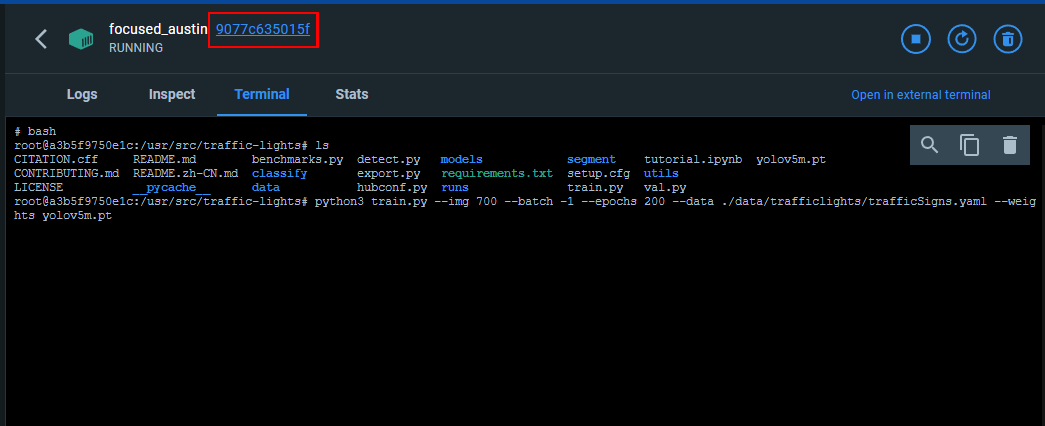
\includegraphics[width=10cm]{data/img/docker_container_terminal.png}
    \caption{Docker Container ausschnitt mit der ID markiert in einem Roten Rahmen}
    \label{fig:doc_cont_term}
\end{figure}

\section{YOLO Modell Trainieren}
Um das Modell zu trainieren sollte in den Docker Container gewechselt werden und das Terminal geöffnet werden. Mit dem Komando \textit{bash} wird in Bash gewechselt und es kann gesehen werden in welchem Ordner man sich befindet. 
\subsection{Befehlserklärung für Training des Modells}
Für das Training des Modells mus in das  Base Directory von dem YOLOv5 Repository gewechselt werden. Darin befindet sich die \textit{train.py} datei. Hierbei kann man das Training mit dem folgenden Befehl starten:
\begin{verbatim}
    python train.py --img <size_of_img> --batch <size_of_batches> --epochs <epochs>
    
    --data <data_path_to_yaml> --weights <weights> [--device <device_numbers> ]
\end{verbatim}
Die in eckickegen Klammern stehende Begriffe sollen nun nochmal erklärt werden:
\begin{itemize}
    \item \textless size\_of\_img\textgreater definiert die Breite des Bildes in Pixel. \textbf{Achtung:} Je höher der Pixelcount, desto höher der RAM / VRAM Verbrauch aber der Anstieg ist nicht linear, sondern Exponentiell
    \item \textless size\_of\_batch\textgreater gibt an wie viele Bilder in einem Durchgang (Epoche) analysiert werden soll. Diese kann per Hand vorgegeben werden, allerdings passiert es dann, dass aufgrund unzureichenden Videospeichers das Training abbricht. Für eine dynamische Anpassung des Videospeichers -1 eingeben. Allerdings kann es sein, dass dann alle Ressourcen genutzt werden.
    \item \textless epochs\textgreater gibt an wie oft trainiert wird. Für jede neue epoche werden die nächsten Batch an Images analysiert bis alle Bilder analysiert sind und der Algorithmus beginnt wieder von vorne. Somit wird sichergestellt, dass bei einer hohen Anzahl an Bildern alle Bilder untersucht werden.
    \item \textless weights\textgreater Für das Training gibt es 5 verschiedene Gewichte: Nano, Small, Medium, Large und XLarge. Für die jeweiligen Gewichte muss folgendes eingegeben werden. Es sei zu beachten, dass mit zunehmender größe die Rechendauer und der Platz an benötigten Arbeitsspeicher massiv zunimmt.
    \begin{itemize}
        \item Nano $\rightarrow $ \textit{yolov5n.pt}
        \item Small $\rightarrow $ \textit{yolov5s.pt}
        \item Medium $\rightarrow $ \textit{yolov5m.pt}
        \item Large $\rightarrow $ \textit{yolov5l.pt}
        \item XLarge $\rightarrow $ \textit{yolov5x.pt}
    \end{itemize}
    \item \textless device\_numbers\textgreater dies ist auch für die Arbeit ein optionaler Parameter. Dieser gibt an welche GPUs genutzt werden sollen. Wird, das ausgelassen geht der Algorithmus von einer CPU Berechnung aus und nutzt den vorliegenden Arbeitsspeicher und die CPU. Damit GPU(s) genutzt werden können müssen die Nummern der GPUs angegeben werden. Diese wird durch das Betriebssystem bestimmt. Wenn nur eine GPU vorhanden ist, ist dies i.d.R. 0. Damit wird der komplette VRAM der GPU genutzt. Voraussetzung dafür ist es, dass das NVIDIA CUDA Toolkit installiert ist und der GPU für den Docker freigeschaltet ist, was jedoch der default ist. Für mehrere GPUs einfach mit Kommata die GPUs auflisten. Für mehr Informationen \textit{\href{https://github.com/ultralytics/yolov5/issues/475}{hier klicken}}.
\end{itemize}

Falls diese Arbeit älter ist ein Jahr oder die bisherigen Angaben funktionieren nicht sei an dieser Stelle auf das Repository von ultralytics verwiesen, die eine ausführliche Dokumentation des Codes haben und all den wichtigen Befehlen.

\subsection{Nach Ausführung}
\label{sec:after_exec}
Nach der Ausführung sollte das Programm im ersten Schritt alle Trainingsdaten einlesen und anschließend je Epoche das Netz trainieren. Egal ob es fertig trainiert hat oder nicht wird in aufsteigender Reihenfolge im Working Directory unter \textit{./data/} zu finden sind. 

Wenn das Trainieren fehlgeschlagen sein sollte enthält der Ordner keine Gewichte. Gewichtsdateien sind mit der Endung \textit{.pt} gekennzeichnet.

Bei erfolgreichem TRainieren werden zwei Dateien Abelegt. Einmal \textit{latest.pt} und \textit{best.pt} die auf den jeweils zuletzt ausgeführten run und den besten run hinweisen. Diese können dann für die spätere Objekterkennung bzw. Ampel und Traffic Signs Erkennung genutzt werden.

